\section*{第二章 平面直角坐标系中的直线}

\section*{一、直线的方程}

\section*{(一) 点斜式和斜截式}

\section*{【典型题型和解题技巧】}

1. 直线斜率的求法.

一般地说, 求直线斜率有三种方法:

(1)利用定义 $k = \tan \alpha$ .

当已知直线的倾斜角为 $\alpha \left( {\alpha  \neq  \dfrac{\pi }{2}}\right)$ 时,可直接利用定义求直线的斜率,即 $k = \tan \alpha$ .

(2)利用“两点式”.

如果直线过两点 $A\left( {{x}_{1},{y}_{1}}\right) ,B\left( {{x}_{2},{y}_{2}}\right) \left( {{x}_{1} \neq  {x}_{2}}\right)$ ,那么可利用公式 $k = \dfrac{{y}_{2} - {y}_{1}}{{x}_{2} - {x}_{1}}$ 来求直线的斜率.

( 3 )利用直线的“斜截式”方程.

如果直线 $l$ 的方程以一般式给出,即 ${ax} + {by} + c = 0\left( {b \neq  0}\right)$ ,那么将 $l$ 的方程化为斜截式, 即 $y =  - \dfrac{a}{b}x - \dfrac{c}{b}$ ,就可以得到直线 $l$ 的斜率为 $- \dfrac{a}{b}$ .

例 1 已知直线 $l$ 过点 $P\left( {2,1}\right)$ ,且与两轴围成等腰直角三角形,求直线 $l$ 的方程.

解 如图 1,此时直线 $l$ 的倾斜角为 $\dfrac{\pi }{4}$ 或 $\dfrac{3\pi }{4},l$ 的斜率为 ${k}_{1} = \tan \dfrac{\pi }{4} = 1,{k}_{2} = \tan \dfrac{3\pi }{4} =  - 1$ ,

故直线 $l$ 的方程为 $y - 1 = 1 \cdot  \left( {x - 2}\right)$ 或 $y - 1 =  - 1 \cdot  \left( {x - 2}\right)$ ,

即 $x - y - 1 = 0$ 或 $x + y - 3 = 0$ .

\begin{center}
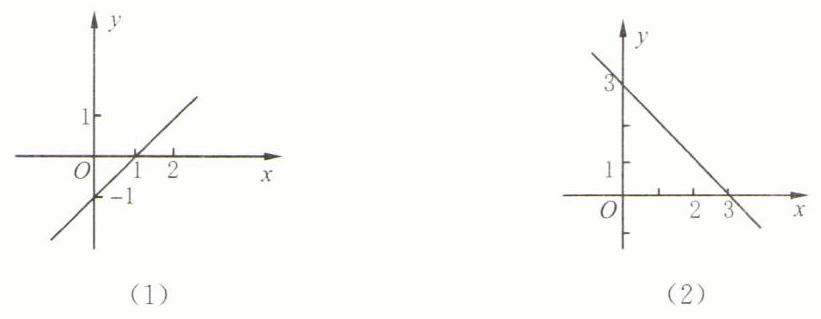
\includegraphics[width=0.7\textwidth]{bodyxb/src/bo_d20aucref24c73anc48g_33_356_1733_821_319_0.jpg}
\end{center}


(图 1)

例 2 已知直线 $l$ 的方程为 $x\sin \theta  - \sqrt{3}y + 2 = 0$ ,当 $\theta$ 在实数范围内变动时,求 $l$ 的倾斜角的取值范围.

解 由已知得 $y = \dfrac{\sin \theta }{\sqrt{3}}x + \dfrac{2}{\sqrt{3}}$ .

\begin{center}
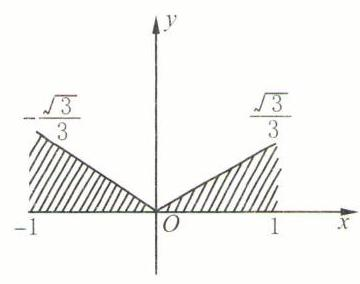
\includegraphics[width=0.3\textwidth]{bodyxb/src/bo_d20aucref24c73anc48g_34_1125_195_360_284_0.jpg}
\end{center}


(图 2)

设直线 $l$ 的倾斜角为 $\alpha$ ,则 $\tan \alpha  = \dfrac{\sin \theta }{\sqrt{3}} \in  \left\lbrack  {-\dfrac{\sqrt{3}}{3},\dfrac{\sqrt{3}}{3}}\right\rbrack$ .

如图 2,易知倾斜角 $\alpha$ 的取值范围是 $\left\lbrack  {0,\dfrac{\pi }{6}}\right\rbrack   \cup  \left\lbrack  {\dfrac{5\pi }{6},\pi }\right)$ .

注意(1)所有的直线都有倾斜角,倾斜角的取值范围是 $\lbrack 0$ , $\pi$ ).

(2)并非所有的直线都有斜率,与 $x$ 轴垂直的直线就不存在斜率.

2. 参数“ $k$ ”.

在直线的 “点斜式” 方程和 “斜截式” 方程中,都有直线的斜率 $k$ ,为了求直线的方程,常常需要确定它的斜率,此时,我们可以把 $k$ 作为未知数引入待定.

例 3 直线 $l$ 过定点 $A\left( {-2,3}\right)$ ,且与两坐标轴围成的三角形面积为 4,求直线 $l$ 的方程.

解 显然, $l$ 不与两坐标轴垂直,设直线 $l$ 的方程为 $y - 3 = k\left( {x + 2}\right)$ .

令 $x = 0$ ,得 $y = {2k} + 3$ ,令 $y = 0$ ,得 $x =  - \dfrac{3}{k} - 2$ ,

于是直线 $l$ 在两轴上的截距分别为 $- \dfrac{3}{k} - 2$ 和 ${2k} + 3$ .

根据题意,得 $\dfrac{1}{2}\left| {\left( {{2k} + 3}\right) \left( {-\dfrac{3}{k} - 2}\right) }\right|  = 4$ ,即 $\left( {{2k} + 3}\right) \left( {\dfrac{3}{k} + 2}\right)  =  \pm  8$ .

若 $\left( {{2k} + 3}\right) \left( {\dfrac{3}{k} + 2}\right)  = 8$ ,化简得 $4{k}^{2} + {4k} + 9 = 0$ ,故 $k \in  \varnothing$ ；

若 $\left( {{2k} + 3}\right) \left( {\dfrac{3}{k} + 2}\right)  =  - 8$ ,化简得 $4{k}^{2} + {20k} + 9 = 0$ ,故 ${k}_{1} =  - \dfrac{1}{2},{k}_{2} =  - \dfrac{9}{2}$ ,

所求直线 $l$ 的方程为 $x + {2y} - 4 = 0$ 和 ${9x} + {2y} + {12} = 0$ .

\section*{【训练题】}

\section*{(A)}

1. 过点 $P\left( {2,3}\right)$ 与 $Q\left( {1,5}\right)$ 的直线 ${PQ}$ 的倾斜角为(   )

(A) arctan2. (B) arctan(-2).

(C) $\dfrac{\pi }{2} + \arctan 2$ . (D) $\pi  - \arctan 2$ .

\begin{center}
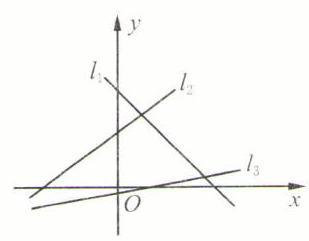
\includegraphics[width=0.2\textwidth]{bodyxb/src/bo_d20aucref24c73anc48g_34_1180_1868_309_241_0.jpg}
\end{center}


(第 2 题)

2. 若图中的直线 ${l}_{1},{l}_{2},{l}_{3}$ 的斜率分别为 ${k}_{1},{k}_{2},{k}_{3}$ ,则有(   )

(A) ${k}_{1} < {k}_{2} < {k}_{3}$ . (B) ${k}_{3} < {k}_{1} < {k}_{2}$ .

(C) ${k}_{3} < {k}_{2} < {k}_{1}$ . (D) ${k}_{1} < {k}_{3} < {k}_{2}$ .

3. 若直线 $l$ 的倾斜角是连接 $\left( {3, - 5}\right) ,\left( {0, - 9}\right)$ 两点的直线倾斜角的 2 倍,则 $l$ 的斜率是 (   )

(A) $\dfrac{24}{25}$ . (B) $\dfrac{8}{3}$ . (C) $- \dfrac{7}{25}$ . (D) $- \dfrac{24}{7}$ .

4. 若三点 $A\left( {3,1}\right) ,B\left( {-2,b}\right) ,C\left( {8,{11}}\right)$ 在同一条直线上,则实数 $b$ 等于(   )

(A) 2 . (B) 3. (C) 9. (D) -9.

5. 直线 ${ax} + {by} = {ab}\left( {a > 0,b < 0}\right)$ 的倾斜角是(   )

(A) $\arctan \left( {-\dfrac{a}{b}}\right)$ . (B) arctan $\dfrac{a}{b}$ .

(C) $\pi  - \arctan \dfrac{a}{b}$ . (D) $\dfrac{\pi }{2} + \arctan \dfrac{a}{b}$ .

6. 过点(1,2),且与原点距离最大的直线方程是(   )

(A) $x + {2y} - 5 = 0$ . (B) ${2x} + y - 4 = 0$ .

(C) $x + {3y} - 7 = 0$ . (D) $x - {2y} + 3 = 0$ .

7. (1)过点 $A\left( {-1,2}\right)$ 且倾斜角的正弦值为 $\dfrac{3}{5}$ 的直线方程是\blkda{}；

(2)已知点 $P\left( {6,a}\right)$ 在过两点 $A\left( {-1,3}\right) ,B\left( {5, - 2}\right)$ 的直线上,则 $a$ 的值等于\blkda{}；

(3)过点(2, - 1)且倾斜角比直线 $x - {3y} + 4 = 0$ 的倾斜角大 ${45}^{ \circ  }$ 的直线方程是\blkda{}；

(4)已知点 $P\left( {2, - 4}\right) ,Q\left( {0,8}\right)$ ,则线段 ${PQ}$ 的垂直平分线方程为\blkda{}；

(5)已知直线 $l$ 过点(3, - 1),且与两坐标轴围成一个等腰直角三角形,则 $l$ 的方程为\blkda{}.

\section*{(B)}

8. 已知直线 $y = \dfrac{1}{2}x + b$ 与 $x$ 轴、 $y$ 轴的交点分别为 $A,B$ . 如果 $\bigtriangleup {AOB}$ 的面积 $(O$ 为原点)小于等于 1,那么 $b$ 的取值范围是(   )

(A) $b \geq   - 1$ . (B) $b \leq  1$ 且 $b \neq  0$ .

(C) $- 1 \leq  b \leq  1$ 且 $b \neq  0$ . (D) $b \leq   - 1$ 或 $b \geq  1$ .

9. 已知点 $M$ 是直线 $l : {2x} - y - 4 = 0$ 与 $x$ 轴的交点,把直线 $l$ 绕点 $M$ 逆时针方向旋转 ${45}^{ \circ  }$ ,则得到的直线方程是(   )

(A) ${3x} + y - 6 = 0$ . (B) ${3x} - y + 6 = 0$ .

(C) $x + y - 2 = 0$ . (D) $x - {3y} - 2 = 0$ .

10. 已知直线 ${l}_{1}$ 的方程是 ${ax} - y + b = 0,{l}_{2}$ 的方程是 ${bx} - y - a = 0\left( {{ab} \neq  0,a \neq  b}\right)$ ,则下列各示意图形中,可能正确的是(   )

\begin{center}
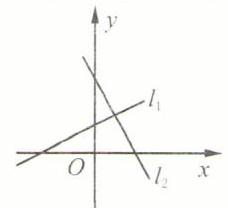
\includegraphics[width=0.2\textwidth]{bodyxb/src/bo_d20aucref24c73anc48g_35_257_1949_228_208_0.jpg}
\end{center}


(A)

\begin{center}
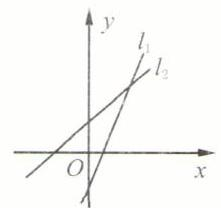
\includegraphics[width=0.2\textwidth]{bodyxb/src/bo_d20aucref24c73anc48g_35_527_1949_221_208_0.jpg}
\end{center}


(B)

\begin{center}
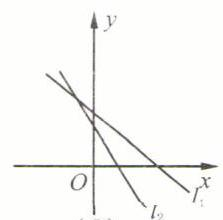
\includegraphics[width=0.2\textwidth]{bodyxb/src/bo_d20aucref24c73anc48g_35_785_1944_223_220_0.jpg}
\end{center}


(C)

\begin{center}
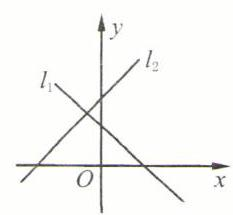
\includegraphics[width=0.2\textwidth]{bodyxb/src/bo_d20aucref24c73anc48g_35_1044_1944_233_215_0.jpg}
\end{center}


(D)

11. 过点(0, - 2)的直线 $l$ 的倾斜角 $\alpha$ 满足 $\sin \dfrac{\alpha }{2} = \dfrac{1}{3}$ ,则 $l$ 的方程是 (   )

(A) $y =  - \dfrac{4\sqrt{2}}{7}x + 2$ . (B) $y =  - \dfrac{4\sqrt{2}}{7}x - 2$ .

(C) $y = \dfrac{4\sqrt{2}}{7}x + 2$ . (D) $y = \dfrac{4\sqrt{2}}{7}x - 2$ .

12. 若 $\theta  \in  \mathbf{R}$ ,则直线 $y = \sin \theta  \cdot  x + 1$ 的倾斜角的取值范围是 (   )

(A) $\left\lbrack  {0,\dfrac{\pi }{2}}\right\rbrack$ . (B) $\left\lbrack  {-\dfrac{\pi }{4},\dfrac{\pi }{4}}\right\rbrack$ .

(C) $\left\lbrack  {\dfrac{\pi }{4},\dfrac{3\pi }{4}}\right\rbrack$ . (D) $\left\lbrack  {0,\dfrac{\pi }{4}}\right\rbrack   \cup  \left\lbrack  {\dfrac{3\pi }{4},\pi }\right)$ .

13. 若 $- \dfrac{\pi }{2} < \theta  < 0$ ,则直线 $y = x\cot \theta$ 的倾斜角等于(   )

(A) $- \theta$ . (B) $\dfrac{\pi }{2} + \theta$ .

(C) $\dfrac{\pi }{2} - \theta$ . (D) $\pi  + \theta$ .

14. 设点 $A\left( {2, - 3}\right) ,B\left( {-3, - 2}\right)$ ,直线 $l$ 过点 $P\left( {1,1}\right)$ 且与线段 ${AB}$ 相交,则 $l$ 的斜率 $k$ 的取值范围是(   )

(A) $k \geq  \dfrac{3}{4}$ 或 $k \leq   - 4$ . (B) $k \geq  \dfrac{3}{4}$ 或 $k \leq   - \dfrac{1}{4}$ .

(C) $- 4 \leq  k \leq  \dfrac{3}{4}$ . (D) $- \dfrac{3}{4} \leq  k \leq  4$ .

15. 若直线 $y = {kx} + b$ 上两点 $P,Q$ 的横坐标分别为 ${x}_{1},{x}_{2}$ ,则 $\left| {PQ}\right|$ 为 (   )

(A) $\left| {{x}_{1} - {x}_{2}}\right|  \cdot  \sqrt{1 + {k}^{2}}$ . (B) $\left| {{x}_{1} - {x}_{2}}\right|  \cdot  \left| k\right|$ .

(C) $\dfrac{\left| {x}_{1} - {x}_{2}\right| }{\sqrt{1 + {k}^{2}}}$ . (D) $\dfrac{\left| {x}_{1} - {x}_{2}\right| }{\left| k\right| }$ .

16. (1) 过原点引直线 $l$ ,使 $l$ 与连接 $A\left( {1,1}\right)$ 和 $B\left( {1, - 1}\right)$ 两点的线段相交,则直线 $l$ 倾斜角的取值范围是\blkda{}；

(2)已知 $A\left( {-\sqrt{3}\sin \theta ,{\cos }^{2}\theta }\right) ,B\left( {0,1}\right)$ 是相异的两点,则直线 ${AB}$ 倾斜角的取值范围是\blkda{}；

(3)若直线的倾斜角 $\alpha$ 满足 $\tan \alpha  \leq  \sqrt{3}$ ,则 $\alpha$ 的取值范围是\blkda{}.

17. (1) 要使三点 $A\left( {2,{\cos }^{2}\theta }\right) ,B\left( {{\sin }^{2}\theta , - \dfrac{2}{3}}\right) ,C\left( {-4, - 4}\right)$ 共线,则角 $\theta$ 的值为\blkda{};

(2)若直线 $y = {ax} + 2$ 与以点 $A\left( {1,4}\right)$ 和 $B\left( {3,1}\right)$ 为端点的线段相交,则 $a$ 的取值范围是\blkda{}；

(3)若直线 $\left( {2{a}^{2} - {7a} + 3}\right) x + \left( {{a}^{2} - 9}\right) y + 3{a}^{2} = 0$ 的倾斜角为 $\dfrac{\pi }{4}$ ,则实数 $a =$ \blkda{}.

18. 已知直线 $l$ 在 $x$ 轴上的截距为 -2,倾斜角 $\alpha$ 满足 $\dfrac{2\sin \alpha  - \cos \alpha }{5\cos \alpha  + 3\sin \alpha } = \dfrac{3}{11}$ ,求直线 $l$ 的方程.

19. 已知 $A\left( {0,0}\right) ,B\left( {8,0}\right) ,C\left( {7,6}\right)$ 是 $\bigtriangleup {ABC}$ 的三个顶点.

(1)求它的外心 $M$ 、垂心 $H$ (即三角形三条高所在直线的交点)、重心 $G$ 的坐标；

(2)求证: $M$ , $H$ , $G$ 三点共线.

20. 已知三点 $A\left( {{x}_{1},{y}_{1}}\right) ,B\left( {{x}_{2},{y}_{2}}\right) ,C\left( {{x}_{3},{y}_{3}}\right)$ ,在坐标平面上求点 $P$ ,使 ${\left| AP\right| }^{2} + {\left| BP\right| }^{2} +$  ${\left| CP\right| }^{2}$ 的值最小.

\section*{(二) 两点式和截距式}

\section*{【典型题型和解题技巧】}

1. 直线截距的求法.

求直线在 $x$ 轴、 $y$ 轴上的截距有两种方法:

(1)把直线的方程化成 “截距式”,即化成 $\dfrac{x}{a} + \dfrac{y}{b} = 1\left( {a \neq  0,b \neq  0}\right)$ ,那么直线在 $x$ 轴、 $y$ 轴上的截距分别是 $a,b$ .

(2)在直线方程中,令 $y = 0$ ,得 $x = {x}_{0}$ ；再令 $x = 0$ ,得 $y = {y}_{0}$ . 故 ${x}_{0},{y}_{0}$ 就是直线在 $x$ 轴、 $y$ 轴上的截距.

例 1 求直线 ${3x} - {4y} = {12}$ 在 $x$ 轴、 $y$ 轴上的截距.

解法一 由已知,将方程化为截距式 $\dfrac{x}{4} + \dfrac{y}{-3} = 1$ ,故直线在 $x$ 轴、 $y$ 轴上的截距分别为 4 和 -3.

解法二 在方程 ${3x} - {4y} = {12}$ 中,令 $y = 0$ ,得 ${x}_{0} = 4$ ; 再令 $x = 0$ ,得 ${y}_{0} =  - 3$ . 故直线在 $x$ 轴、 $y$ 轴上的截距分别为 4 和 -3 .

例 2 已知直线 $x - {2y} + {2k} = 0$ 与两坐标轴围成的三角形面积不大于 1,求 $k$ 的取值范围.

解 令 $y = 0$ ,得 $x =  - {2k}$ ; 令 $x = 0$ ,得 $y = k$ . 于是三角形的面积 $S = \dfrac{1}{2}\left| {-{2k}}\right|  \cdot  \left| k\right|  = {k}^{2}$ . 由题意得 $0 < {k}^{2} \leq  1,\therefore  - 1 \leq  k \leq  1$ 且 $k \neq  0$ .

2. 直线方程与不等式.

\begin{center}
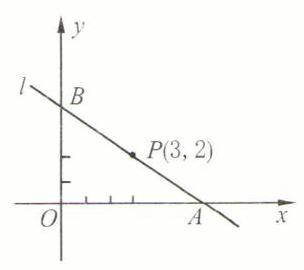
\includegraphics[width=0.2\textwidth]{bodyxb/src/bo_d20aucref24c73anc48g_37_1110_1686_304_270_0.jpg}
\end{center}


(图 3)

例 3 已知直线 $l$ 过点 $P\left( {3,2}\right)$ ,且与 $x$ 轴正半轴、 $y$ 轴正半轴分别交于点 $A,B$ (如图 3).

(1)求 $\bigtriangleup {AOB}$ 面积的最小值及此时 $l$ 的方程( $O$ 为坐标原点)；

(2)求直线 $l$ 在两坐标轴上截距之和的最小值.

(1)解法一 设点 $A,B$ 的坐标依次为 $\left( {a,0}\right) ,\left( {0,b}\right)$ (显然 $a > 3$ ),则直线 $l$ 的方程为 $\dfrac{x}{a} +$  $\dfrac{y}{b} = 1$ . 将 $P\left( {3,2}\right)$ 代入,得 $\dfrac{3}{a} + \dfrac{2}{b} = 1$ ,于是 $b = \dfrac{2a}{a - 3}$ ,

故 $\bigtriangleup  {AOB}$ 的面积 $S = \dfrac{1}{2}{ab} = \dfrac{{a}^{2}}{a - 3} = \dfrac{{\left( a - 3\right) }^{2} + 6\left( {a - 3}\right)  + 9}{a - 3} = \left( {a - 3}\right)  + \dfrac{9}{a - 3} + 6 \geq$  $2\sqrt{\left( {a - 3}\right)  \cdot  \dfrac{9}{a - 3}} + 6 = {12},$

$\therefore$ 当 $a - 3 = \dfrac{9}{a - 3}$ ,即 $a = 6,b = 4$ 时, $\bigtriangleup  {AOB}$ 的面积取最小值 12 ,此时 $l$ 的方程为 $\dfrac{x}{6} + \dfrac{y}{4}$  $= 1$ ,即 ${2x} + {3y} - {12} = 0$ .

解法二 由 $1 = \dfrac{3}{a} + \dfrac{2}{b} \geq  2\sqrt{\dfrac{6}{ab}}$ ,得 $\sqrt{ab} \geq  2\sqrt{6}$ ,

$\therefore {ab} \geq  {24}$ ,故面积 $S = \dfrac{1}{2}{ab} \geq  {12}$ .

$\therefore$ 当 $\dfrac{3}{a} = \dfrac{2}{b} = \dfrac{1}{2}$ ,即 $a = 6,b = 4$ 时, ${S}_{\text{ 最小值 }} = {12}$ . 直线方程同解法一.

解法三 由 $b = \dfrac{2a}{a - 3}$ ,得 $S = \dfrac{1}{2}{ab} = \dfrac{{a}^{2}}{a - 3}$ ,去分母得, ${a}^{2} - {Sa} + {3S} = 0$ .

$\because a$ 为实数, $\therefore \Delta  \geq  0$ ,即 ${S}^{2} - {12S} \geq  0$ . 又 $S \geq  0$ ,于是得 $S \geq  {12}$ .

将 ${S}_{\text{ 最小值 }} = {12}$ 代入上式,求得 $a = 6$ ,故 $b = 4$ . 直线方程同解法一.

解法四 如图 4,过点 $P$ 分别作 $x$ 轴、 $y$ 轴的垂线 ${PM},{PN}(M,N$ 为垂足),并设 $\theta  = \angle {PAM} = \angle {BPN}$ ,则

\begin{center}
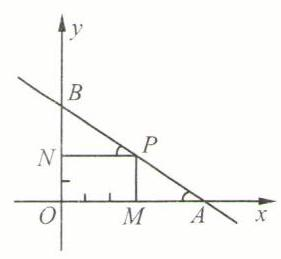
\includegraphics[width=0.2\textwidth]{bodyxb/src/bo_d20aucref24c73anc48g_38_1203_1215_281_259_0.jpg}
\end{center}


(图 4)

$S = {S}_{\text{ 四边形 OMPN }} + {S}_{\bigtriangleup {PAM}} + {S}_{\bigtriangleup {PBN}} = 6 + \dfrac{1}{2} \cdot  2 \cdot  2\cot \theta  + \dfrac{1}{2} \cdot  3 \cdot  3\tan \theta$  $= 6 + 2\cot \theta  + \dfrac{9}{2}\tan \theta  \geq  6 + 2\sqrt{2\cot \theta  \cdot  \dfrac{9}{2}\tan \theta } = {12}$ ,

$\therefore$ 当 $2\cot \theta  = \dfrac{9}{2}\tan \theta$ ,即 $\tan \theta  = \dfrac{2}{3}$ 时, ${S}_{\text{ 最小值 }} = {12}$ . 直线方程同解法一.

(2)解法一 ∵ $\dfrac{3}{a} + \dfrac{2}{b} = 1$ .

$\therefore a + b = \left( {\dfrac{3}{a} + \dfrac{2}{b}}\right) \left( {a + b}\right)  = 3 + \dfrac{3b}{a} + \dfrac{2a}{b} + 2 = 5 + \dfrac{3b}{a} + \dfrac{2a}{b} \geq  5 + 2\sqrt{\dfrac{3b}{a} \cdot  \dfrac{2a}{b}} = 5 + 2\sqrt{6}$ ,

$\therefore$ 当 $\dfrac{3b}{a} = \dfrac{2a}{b}$ ,即 $a = 3 + \sqrt{6},b = 2 + \sqrt{6}$ 时, ${\left( a + b\right) }_{\text{ 最小值 }} = 5 + 2\sqrt{6}$ .

解法二 如图 4, $\because a + b = \left( {\left| {OM}\right|  + \left| {MA}\right| }\right)  + \left( {\left| {ON}\right|  + \left| {NB}\right| }\right)  = \left( {3 + 2\cot \theta }\right)  + (2 +$  $3\tan \theta ) = 5 + 2\cot \theta  + 3\tan \theta  \geq  5 + 2\sqrt{2\cot \theta  \cdot  3\tan \theta } = 5 + 2\sqrt{6}$ ,

$\therefore$ 当 $2\cot \theta  = 3\tan \theta$ ,即 $\tan \theta  = \dfrac{\sqrt{6}}{3}$ ,即 $a = 3 + \sqrt{6},b = 2 + \sqrt{6}$ 时, $\left( {a + b}\right)$ 最小值 $= 5 + 2\sqrt{6}$ .

\section*{(A)}

21. 在 $x$ 轴、 $y$ 轴上的截距分别是 -2,3 的直线方程是(   )

(A) ${3x} - {2y} + 6 = 0$ . (B) ${3x} + {2y} + 1 = 0$ .

(C) ${3x} - {2y} - 6 = 0$ . (D) ${3x} - {2y} + 1 = 0$ .

22. 若直线 $\left( {m + 2}\right) x + \left( {{m}^{2} - {2m} - 3}\right) y = {2m}$ 在 $x$ 轴上的截距是 3,则实数 $m$ 的值等于(   )

(A) $- \dfrac{6}{5}$ . (B) $\dfrac{6}{5}$ . (C)-6. (D) 6.

23. 直线 ${3x} - {2y} = 4$ 的截距式方程是(   )

(A) $\dfrac{3x}{4} - \dfrac{y}{2} = 1$ . (B) $\dfrac{x}{\dfrac{1}{3}} - \dfrac{y}{\dfrac{1}{2}} = 4$ .

(C) $\dfrac{3x}{4} + \dfrac{y}{-2} = 1$ . (D) $\dfrac{x}{\dfrac{4}{3}} + \dfrac{y}{-2} = 1$ .

24. 过点(3, - 4)且在两坐标轴上的截距相等的直线方程是 (   )

(A) $x + y + 1 = 0$ . (B) ${4x} - {3y} = 0$ .

(C) ${4x} + {3y} = 0$ . (D) ${4x} + {3y} = 0$ 或 $x + y + 1 = 0$ .

25. (1) 若直线与两坐标轴相交且被两坐标轴截得的线段中点是(2,4),则此直线的方程为\blkda{}；

(2)若直线在两坐标轴上的截距之和为 2 且经过点(-2,3),则此直线的方程为\blkda{}；

(3) 若直线 $\dfrac{a}{3}x - {2y} - {4a} = 0\left( {a \neq  0}\right)$ 在 $x$ 轴上的截距是它在 $y$ 轴上截距的 3 倍,则 $a$  $=$ \blkda{}.

26. 已知直线的斜率为 $\dfrac{1}{6}$ ,且和两坐标轴围成的三角形面积为 3,求此直线的方程.

27. 在 $\bigtriangleup {ABC}$ 中,已知点 $A\left( {5, - 2}\right) ,B\left( {7,3}\right)$ ,且边 ${AC}$ 的中点 $M$ 在 $y$ 轴上,边 ${BC}$ 的中点 $N$ 在 $x$ 轴上. 求: (1) 顶点 $C$ 的坐标; (2) 直线 ${MN}$ 的方程.

\section*{(B)}

28. 已知点 $M\left( {1,3}\right) ,N\left( {5, - 2}\right)$ ,在 $x$ 轴上取一点 $P$ ,使 $\left| \right| {PM}\left| -\right| {PN}\left| \right|$ 最大,则点 $P$ 的坐标是(   )

(A)(3.4,0). (B)(5,0).

(C)(13,0). (D)(0,13).

29. 下列说法正确的是(   )

(A) $\dfrac{y - {y}_{1}}{x - {x}_{1}} = k$ 表示过点 ${P}_{1}\left( {{x}_{1},{y}_{1}}\right)$ 且斜率为 $k$ 的直线方程.

(B) 直线 $y = {kx} + b$ 与 $y$ 轴交于一点 $B\left( {0,b}\right)$ ,其中 $b = \left| {OB}\right|$ .

(C) 若直线在 $x$ 轴和 $y$ 轴上的截距分别为 $a$ 与 $b$ ,则直线的方程是 $\dfrac{x}{a} + \dfrac{y}{b} = 1$ .

(D) 方程 $\left( {{x}_{2} - {x}_{1}}\right) \left( {y - {y}_{1}}\right)  = \left( {{y}_{2} - {y}_{1}}\right) \left( {x - {x}_{1}}\right)$ (其中 ${x}_{1} \neq  {x}_{2}$ 或 ${y}_{1} \neq  {y}_{2}$ ) 表示过两点 ${P}_{1}\left( {{x}_{1},{y}_{1}}\right) ,{P}_{2}\left( {{x}_{2},{y}_{2}}\right)$ 的一条直线.

30. 已知三条直线为 ${l}_{1} : x - {2y} + {4a} = 0,{l}_{2} : x - y - {6a} = 0,{l}_{3} : {2x} - y - {4a} = 0\left( {a \neq  0}\right)$ ,则下列结论中正确的是(   )

(A) 三条直线的倾斜角之和为 ${90}^{ \circ  }$ .

(B) 三条直线在 $y$ 轴上的截距 ${b}_{1},{b}_{2},{b}_{3}$ 满足 ${b}_{1} + {b}_{3} = 2{b}_{2}$ .

(C) 三条直线的倾斜角 ${\alpha }_{1},{\alpha }_{2},{\alpha }_{3}$ 满足 ${\alpha }_{1} + {\alpha }_{3} = 2{\alpha }_{2}$ .

(D) 三条直线在 $x$ 轴上的截距之和为 ${12}\left| a\right|$ .

31. (1) 已知直线 $l$ 的倾斜角为 $\alpha  = \arccos \left( {-\dfrac{4}{5}}\right)$ ,它在两坐标轴上的截距之和为 1,求直线 $l$ 的方程;

(2)已知直线 $l$ 与两坐标轴围成一个等腰直角三角形,且此三角形的面积为 18,求直线 $l$ 的方程;

(3)已知直线 $l$ 过点 $P\left( {-4,3}\right)$ ,与 $x$ 轴、 $y$ 轴分别交于 $A,B$ 两点,且 $\left| {AP}\right|  : \left| {PB}\right|  = 5$ : 3,求直线 $l$ 的方程;

(4)已知 $A\left( {1,1}\right) ,B\left( {5,3}\right) ,C\left( {4,5}\right)$ 是 $\bigtriangleup {ABC}$ 的三个顶点,直线 $l//{AB}$ 且平分 $\bigtriangleup {ABC}$ 的面积,求直线 $l$ 的方程.

32. 已知定点 $P\left( {6,4}\right)$ 及定直线 $l : y = {4x}$ ,点 $Q$ 在直线 $l$ 上 ( $Q$ 在第一象限),直线 ${PQ}$ 交 $x$ 轴正半轴于点 $M$ . 要使 $\bigtriangleup {OMQ}$ 的面积最小 $(O$ 为原点),求点 $Q$ 的坐标.

\section*{(三) 直线方程的一般形式}

\section*{【典型题型和解题技巧】}

1. 直线方程形式. 续表

\begin{center}
\adjustbox{width=\textwidth}{
\begin{tabular}{|c|c|c|}
\hline
方程名称 & 方程形式 & 方程的缺陷 \\
\cline{1-3}
点斜式 & $y - {y}_{0} = k\left( {x - {x}_{0}}\right)$ & 不包括与 $x$ 轴垂直的直线 \\
\cline{1-3}
斜截式 & $y = {kx} + b$ & 不包括与 $x$ 轴垂直的直线 \\
\cline{1-3}
两点式 & $\dfrac{x - {x}_{1}}{{x}_{2} - {x}_{1}} = \dfrac{y - {y}_{1}}{{y}_{2} - {y}_{1}}$  $\left( {{x}_{1} \neq  {x}_{2},{y}_{1} \neq  {y}_{2}}\right)$ & 不包括与 $x$ 轴垂直、与 $y$ 轴垂直的直线 \\
\cline{1-3}
\hline
\end{tabular}
}
\end{center}

\begin{center}
\adjustbox{width=\textwidth}{
\begin{tabular}{|c|c|c|}
\hline
方程名称 & 方程形式 & 方程的缺陷 \\
\cline{1-3}
截距式 & $\dfrac{x}{a} + \dfrac{y}{b} = 1$  $\left( {a \neq  0,b \neq  0}\right)$ & 不包括与 $x$ 轴垂直、与 $y$ 轴垂直、过原点的直线 \\
\cline{1-3}
一般式 & ${Ax} + {By} + C = 0$ ( $A,B$ 不同时为零) & \phantom{X} \\
\cline{1-3}
\hline
\end{tabular}
}
\end{center}

2. 一般式与斜截式.

若直线 $l$ 的方程是一般式 ${ax} + {by} + c = 0$ ,则当 $b \neq  0$ 时,可以化成斜截式 $y =  - \dfrac{a}{b}x - \dfrac{c}{b}$ .

例 1 如果 ${pr} < 0,{qr} < 0$ ,那么直线 ${px} + {qy} + r = 0$ 不通过 (   )

(A)第一象限. (B)第二象限. (C) 第三象限. (D) 第四象限.

解 显然 $q \neq  0$ ,由已知直线方程得 $y =  - \dfrac{p}{q}x - \dfrac{r}{q}$ .

\begin{center}
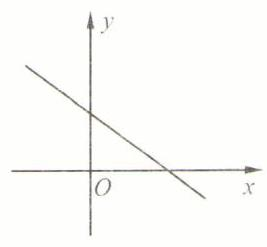
\includegraphics[width=0.2\textwidth]{bodyxb/src/bo_d20aucref24c73anc48g_41_1155_801_267_247_0.jpg}
\end{center}


(图 5)

$\because {qr} < 0,\therefore  - \dfrac{r}{q} > 0$ ,故直线与 $y$ 轴正半轴相交. 又 ${pr} < 0$ ,故 $p,q$ 同号,则 $- \dfrac{p}{q} < 0$ ,故直线的倾斜角是钝角. 因此,直线如图 5 所示,它不通过第三象限,故选 C.

3. 直线标点法.

借助直线的方程, 用一个量 (字母) 来表示直线上点的两个坐标, 这种方法称为 “直线标点法”.

例 2 在直线 ${3x} - y + 1 = 0$ 上确定一点 $P$ ,使点 $P$ 到两点 $\left( {1, - 1}\right) ,\left( {2,0}\right)$ 的距离相等.

解 $\because$ 点 $P$ 在直线 ${3x} - y + 1 = 0$ 上,故可设点 $P$ 的坐标为 $\left( {a,{3a} + 1}\right)$ ,

则有 ${\left( a - 1\right) }^{2} + {\left\lbrack  \left( 3a + 1\right)  - \left( -1\right) \right\rbrack  }^{2} = {\left( a - 2\right) }^{2} + {\left( 3a + 1\right) }^{2}$ ,

化简得 $a = 0$ ,于是点 $P$ 的坐标为(0,1).

\section*{【训练题】}

\section*{(A)}

33. 在平面直角坐标系中,直线 $x + \sqrt{3}y + 1 = 0$ 的倾斜角等于 (   )

(A) $\dfrac{\pi }{6}$ . (B) $\dfrac{\pi }{3}$ . (C) $\dfrac{2\pi }{3}$ . (D) $\dfrac{5}{6}\pi$ .

34. 若 $a,b,c$ 都是正数,则直线 ${ax} + {by} + c = 0$ 的图像大致是 (   )

\begin{center}
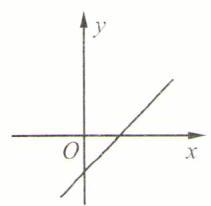
\includegraphics[width=0.2\textwidth]{bodyxb/src/bo_d20aucref24c73anc48g_41_288_1944_211_206_0.jpg}
\end{center}


(A)

\begin{center}
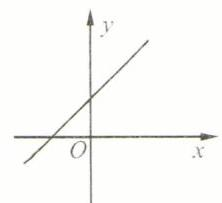
\includegraphics[width=0.2\textwidth]{bodyxb/src/bo_d20aucref24c73anc48g_41_522_1944_222_203_0.jpg}
\end{center}


(B)

\begin{center}
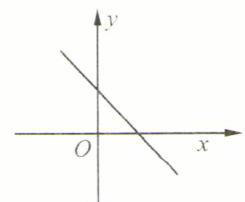
\includegraphics[width=0.2\textwidth]{bodyxb/src/bo_d20aucref24c73anc48g_41_768_1944_245_202_0.jpg}
\end{center}


(C)

\begin{center}
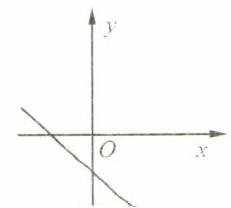
\includegraphics[width=0.2\textwidth]{bodyxb/src/bo_d20aucref24c73anc48g_41_1035_1942_231_208_0.jpg}
\end{center}


(D)

35. 若 ${ab} < 0,{bc} < 0$ ,则直线 ${ax} + {by} + c = 0$ 通过(   )

(A) 第一、二、三象限. (B) 第一、二、四象限. (D) 第二、三、四象限. (C) 第一、三、四象限.

\section*{(B)}

36. 若 ${ab} < 0$ ,则直线 ${ax} - {by} - c = 0$ 的倾斜角的取值范围是(   )

(A) $\left( {0,\dfrac{\pi }{2}}\right)$ . (B) $\left( {\dfrac{\pi }{2},\pi }\right)$ .

(C) $\left( {-\pi , - \dfrac{\pi }{2}}\right)$ . (D) $\left( {-\dfrac{\pi }{2},0}\right)$ .

37. 若直线 ${ax} - y + 2 = 0$ 与直线 ${3x} - y - b = 0$ 关于直线 $y = x$ 对称,则 $a,b$ 的值为(   )

(A) $a = \dfrac{1}{3},b = 6$ . (B) $a = \dfrac{1}{3},b =  - 6$ .

(C) $a = 3,b =  - 2$ . (D) $a = 3,b = 6$ .

38. 由方程 $\left| {x - 1}\right|  + \left| {y - 1}\right|  = 1$ 确定的曲线所围成的图形的面积为(   ) (D) 8. (A) 1 . (B) 2 . (C) 4.

39. 设全集 $U = \{ \left( {x,y}\right)  \mid  x,y \in  \mathbf{R}\} ,M = \left\{  {\left( {x,y}\right) \left| {\dfrac{y - 3}{x - 2} = 1}\right. }\right\}  ,N = \{ \left( {x,y}\right)  \mid  y \neq  x + 1\}$ ,则 $\overline{M \cup  N}$ 等于(   )

(A) $\varnothing$ . (B) $\{ \left( {2,3}\right) \}$ . (D) $\{ \left( {x,y}\right)  \mid  y = x + 1\}$ . (C)(2,3).

40. (1) 与直线 $x - y + \sqrt{3} = 0$ 关于原点成中心对称的直线方程是\blkda{}；

(2)若直线 $l$ 与直线 $y = {ax} + b\left( {a \neq  0}\right)$ 夹角的平分线是直线 $y = x$ ,则直线 $l$ 的方程是\blkda{}.

41. 若动点 $A\left( {{x}_{1},{y}_{1}}\right) ,B\left( {{x}_{2},{y}_{2}}\right)$ 分别在直线 $x + y - 7 = 0$ 和直线 $x +$  $y - 5 = 0$ 上,求 ${AB}$ 的中点 $M$ 到原点距离的最小值.

\begin{center}
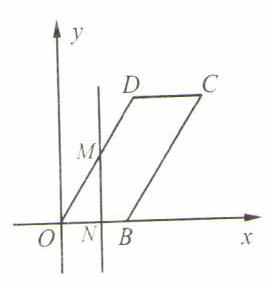
\includegraphics[width=0.2\textwidth]{bodyxb/src/bo_d20aucref24c73anc48g_42_1248_1436_270_284_0.jpg}
\end{center}


(第 42 题)

42. 已知四边形 ${OBCD}$ 是平行四边形, $\left| {OB}\right|  = 1,\left| {OD}\right|  = 2,\angle {BOD} =$  ${60}^{ \circ  }$ ,动直线 $x = t$ 由 $y$ 轴起向右平移,分别交平行四边形两边于不同的两点 $M,N$ (如图).

(1)求点 $D$ 和 $C$ 的坐标,写出用 $t$ 表示 $\bigtriangleup {OMN}$ 的面积表达式 $S\left( t\right)$ ；

(2)当 $t$ 为何值时, $S\left( t\right)$ 有最大值？并求此最大值.

\section*{二、两条直线的位置关系}

\section*{(一) 两条直线的平行与垂直}

\section*{【典型题型和解题技巧】}

1. 参数法求与直线 $l$ 平行或垂直的直线方程.

如果直线 $l$ 的方程是 ${ax} + {by} + c = 0$ ,那么,与 $l$ 平行的直线可以设为: ${ax} + {by} + m = 0(m$  $\neq  c$ )；与 $l$ 垂直的直线可以设为: ${bx} - {ay} + n = 0$ . 其中 $m$ , $n$ 称为待定的 “参数”.

例 1 已知直线 $l$ 的方程为 ${3x} + {4y} - {12} = 0$ ,求直线 ${l}^{\prime }$ 的方程,使得:

(1) ${l}^{\prime }$ 与 $l$ 平行,且过点(-1,3)；

(2) ${l}^{\prime }$ 与 $l$ 垂直,且 ${l}^{\prime }$ 与两坐标轴围成的三角形面积为 4.

解(1)由条件,可设 ${l}^{\prime }$ 的方程为 ${3x} + {4y} + m = 0$ .

将 $x =  - 1,y = 3$ 代入,得 $- 3 + {12} + m = 0$ ,即得 $m =  - 9$ ,

$\therefore$ 直线 ${l}^{\prime }$ 的方程是 ${3x} + {4y} - 9 = 0$ .

(2)由条件,可设 ${l}^{\prime }$ 的方程为 ${4x} - {3y} + n = 0$ .

令 $y = 0$ ,得 $x =  - \dfrac{n}{4}$ ; 令 $x = 0$ ,得 $y = \dfrac{n}{3}$ .

于是由三角形面积 $S = \dfrac{1}{2} \cdot  \left| {-\dfrac{n}{4}}\right|  \cdot  \left| \dfrac{n}{3}\right|  = 4$ ,得 ${n}^{2} = {96},\therefore n =  \pm  4\sqrt{6}$ ,

$\therefore$ 直线 ${l}^{\prime }$ 的方程是 ${4x} - {3y} + 4\sqrt{6} = 0$ 或 ${4x} - {3y} - 4\sqrt{6} = 0$ .

2. 两条直线垂直的条件.

如果两条直线 ${l}_{1}$ 和 ${l}_{2}$ 的方程分别为 ${A}_{1}x + {B}_{1}y + {C}_{1} = 0$ 和 ${A}_{2}x + {B}_{2}y + {C}_{2} = 0\left( {{A}_{1},{B}_{1}}\right.$ 不全为零, ${A}_{2},{B}_{2}$ 不全为零),那么 ${l}_{1} \bot  {l}_{2}$ 的条件是 ${A}_{1}{A}_{2} + {B}_{1}{B}_{2} = 0$ .

例 2 如果直线 ${l}_{1} : \left( {2{m}^{2} + m - 3}\right) x + \left( {{m}^{2} - m}\right) y = {4m} - 1$ 与直线 ${l}_{2} : x - {3y} - 5 = 0$ 互相垂直,求 $m$ 的值.

解 由已知,得 $1 \cdot  \left( {2{m}^{2} + m - 3}\right)  + \left( {-3}\right) \left( {{m}^{2} - m}\right)  = 0$ ,即 ${m}^{2} - {4m} + 3 = 0$ ,于是 $m = 1$ 或 $m = 3$ .

当 $m = 1$ 时,直线 ${l}_{1}$ 的方程为 $0 = 3$ ,显然不合要求, $\therefore m = 3$ .

3. 轴对称.

容易知道,点 $P\left( {a,b}\right)$ 关于 $x$ 轴对称的点是(a, - b); 关于 $y$ 轴对称的点是(-a, b); 关于直线 $x - y = 0$ 对称的点是(b, a); 关于直线 $x + y = 0$ 对称的点是(-b, - a).

一般地,设点 $P\left( {m,n}\right)$ 关于直线 ${ax} + {by} + c = 0$ 对称的点为 $Q\left( {{x}_{0},{y}_{0}}\right)$ ,那么 $\left( {{x}_{0},{y}_{0}}\right)$ 应满

足方程组 $\left\{  \begin{array}{l} \dfrac{{y}_{0} - n}{{x}_{0} - m} \cdot  \left( {-\dfrac{a}{b}}\right)  =  - 1\left( {b \neq  0}\right) , \\  a \cdot  \dfrac{{x}_{0} + m}{2} + b \cdot  \dfrac{{y}_{0} + n}{2} + c = 0. \end{array}\right.$

例 3 求点 $P\left( {2,3}\right)$ 关于直线 $l : {2x} - y - 4 = 0$ 的对称点 $Q$ .

解 设点 $Q\left( {a,b}\right)$ . 由 ${PQ}\bot l$ 且 ${PQ}$ 被 $l$ 平分,有 $\left\{  \begin{array}{l} \dfrac{b - 3}{a - 2} \times  2 =  - 1, \\  2 \times  \dfrac{a + 2}{2} - \dfrac{b + 3}{2} - 4 = 0. \end{array}\right.$

解得 $a = \dfrac{22}{5},b = \dfrac{9}{5}.\therefore $ 点 $Q$ 的坐标为 $\left( {\dfrac{22}{5},\dfrac{9}{5}}\right)$ .

4. 入射光线和反射光线问题.

例 4 光线通过点 $A\left( {-2,4}\right)$ ,遇直线 $l : {2x} - y - 7 = 0$ 后反射. 若反射光线通过点 $B\left( {5,8}\right)$ , 求入射光线和反射光线所在直线的方程.

解 如图 6,设光线经 $l$ 上点 $C$ 反射,则 $\angle 1 = \angle 2$ .

\begin{center}
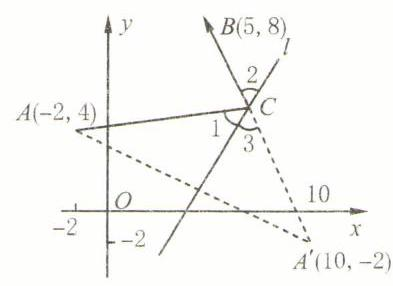
\includegraphics[width=0.3\textwidth]{bodyxb/src/bo_d20aucref24c73anc48g_44_1040_667_393_286_0.jpg}
\end{center}


(图 6)

设点 $A$ 关于 $l$ 对称的点为 ${A}^{\prime }$ ,则 $\angle 1 = \angle 3$ .

$\therefore \angle 2 = \angle 3$ ,故 $B,C,{A}^{\prime }$ 三点共线.

易得点 ${A}^{\prime }$ 的坐标为(10, - 2),

则直线 ${A}^{\prime }B$ 的方程为 ${2x} + y - {18} = 0$ .

解方程组 $\left\{  \begin{array}{l} {2x} + y - {18} = 0, \\  {2x} - y - 7 = 0, \end{array}\right.$ 得点 $C$ 的坐标为 $\left( {\dfrac{25}{4},\dfrac{11}{2}}\right)$ ,则直线 ${AC}$ 的方程为 ${2x} - {11y} + {48} = 0$ .

$\therefore$ 入射光线所在的直线方程为 ${2x} - {11y} + {48} = 0$ ,反射光线所在直线方程为 ${2x} + y - {18}$  $= 0$ .

注意 若将此例改为在直线 $l$ 上求一点 $C$ ,使 $\left| {AC}\right|  + \left| {BC}\right|$ 为最小,解法与上类同,只需先求点 $A$ 关于 $l$ 的对称点 ${A}^{\prime }$ ,则直线 ${A}^{\prime }B$ 与直线 $l$ 的交点即为所求.

\section*{【训练题】}

\section*{(A)}

43. 已知直线 ${l}_{1} : x + {my} + 6 = 0$ 和 ${l}_{2} : \left( {m - 2}\right) x + {3y} + {2m} = 0$ 互相平行,则实数 $m$ 只能是(   )

(A) $m =  - 1$ 或 $m = 3$ . (B) $m =  - 1$ .

(C) $m =  - 3$ . (D) $m = 1$ 或 $m =  - 3$ .

44. 直线 $x + y - 4 = 0$ 上的点与坐标原点的距离的最小值是 (   )

(A) $\sqrt{10}$ . (B) $2\sqrt{2}$ .

(C) $\sqrt{6}$ . (D) 2 .

45. 以 $A\left( {1,3}\right) ,B\left( {-5,1}\right)$ 为端点的线段的垂直平分线的方程是 (   )

(A) ${3x} - y - 8 = 0$ . (B) ${3x} + y + 4 = 0$ .

(C) ${3x} - y + 6 = 0$ . (D) ${3x} + y + 2 = 0$ .

46. 已知直线 $l$ 平行于直线 ${3x} + {4y} - 5 = 0$ ,且直线 $l$ 和两坐标轴在第一象限内所围成的三角形面积是 24,则直线 $l$ 的方程是 (   )

(A) ${3x} + {4y} - {12}\sqrt{2} = 0$ . (B) ${3x} + {4y} + {12}\sqrt{2} = 0$ .

(C) ${3x} + {4y} - {24} = 0$ . (D) ${3x} + {4y} + {24} = 0$ .

47. 在三角形中,已知三边 $a,b,c$ 对应的三内角 $\alpha ,\beta ,\gamma$ 满足 $\lg \sin \alpha  + \lg \sin \gamma  = 2\lg \sin \beta$ ,则直线 $x{\sin }^{2}\alpha  + y\sin \alpha  = a$ 与 $x{\sin }^{2}\beta  + y\sin \gamma  = c$ 的位置关系是(   )

(A) 平行. (B) 斜交. (C) 垂直. (D) 重合.

48. 点(a, b)关于直线 $x + y = 0$ 对称的点是 (   )

(A)(-a, - b). (B)(a, - b).

(C)(b, a). (D)(-b, - a).

49. (1) 已知直线 ${l}_{1} : {px} + {3y} + 1 = 0$ 和 ${l}_{2} : {6x} + {2y} - 5 = 0$ .

①若 ${l}_{1}//{l}_{2}$ ,则 $p =$ \blkda{}, ②若 ${l}_{1} \bot  {l}_{2}$ ,则 $p =$ \blkda{}；

(2)给定三点 $A\left( {1,0}\right)$ , $B\left( {-1,0}\right)$ , $C\left( {1,2}\right)$ ,那么通过点 $A$ 且与直线 ${BC}$ 垂直的直线方程是\blkda{}；

(3)若点(1,2)在直线 $l$ 上的射影为(-1,4),则直线 $l$ 的方程为\blkda{}；

(4) 过点(3,5)的所有直线中,距原点最远的直线方程是\blkda{}；

(5) 若直线 $\left( {2{m}^{2} + m - 3}\right) x + \left( {{m}^{2} - m}\right) y = {4m} - 1$ 与直线 ${2x} - {3y} = 5$ 互相平行,则实数 $m$ 的值等于\blkda{}；

(6)若直线 ${2x} - {5y} + {20} = 0$ 和 ${mx} - {2y} - {10} = 0$ 与两坐标轴围成的四边形有一个外接圆, 则实数 $m$ 的值等于\blkda{}；

(7)若直线 $l$ 过点(-1,2),且在 $x$ 轴上的截距是 -4,则过点(a, b)且垂直于已知直线 $l$ 的直线方程是\blkda{}.

\section*{(B)}

50. 若直线 ${l}_{1} : {ax} + \left( {1 - a}\right) y = 3$ 与直线 ${l}_{2} : \left( {a - 1}\right) x + \left( {{2a} + 3}\right) y = 2$ 互相垂直,则 $a$ 的值是(   )

(A)-3. (B) 1 .

(C) 0 或 $- \dfrac{3}{2}$ . (D) 1 或 -3 .

51. 点(4,0)关于直线 ${5x} + {4y} + {21} = 0$ 对称的点是(   )

(A)(-6,8). (B)(-8, - 6).

(C)(6,8). (D)(-6, - 8).

52. 已知直线 ${l}_{1} : {ax} + {by} + {2a} = 0$ 及 ${l}_{2} : \left( {a - 1}\right) x + y + b = 0$ 满足下列条件,分别求 $a,b$ 的值:

(1)两直线都平行于直线 $x + {2y} + 3 = 0$ ；

(2)两直线互相垂直,且 ${l}_{1}$ 过点(-1,1).

53. (1) 已知 $A\left( {2,3}\right) ,B\left( {6,6}\right)$ 是正方形 ${ABCD}$ 的相邻两个顶点 $(A,B,C,D$ 按顺时针方向排列),求另两个顶点 $C,D$ 的坐标 (如图);

\begin{center}
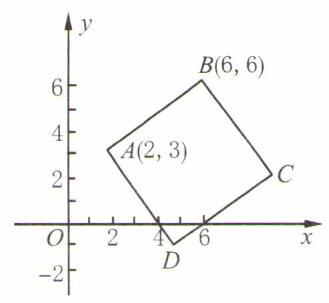
\includegraphics[width=0.2\textwidth]{bodyxb/src/bo_d20aucref24c73anc48g_46_400_280_329_303_0.jpg}
\end{center}


[第 53(1)题]

\begin{center}
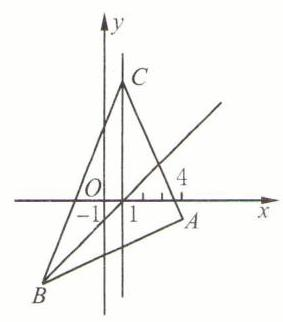
\includegraphics[width=0.2\textwidth]{bodyxb/src/bo_d20aucref24c73anc48g_46_989_259_283_322_0.jpg}
\end{center}


[第 53(6)题]

(2)若点 $A\left( {a + 2,b + 2}\right)$ 关于直线 ${4x} + {3y} + {11} = 0$ 对称的点是 $B\left( {b - 4,a - b}\right)$ ,求 $a$ , $b$ 的值;

(3)光线由点 $P\left( {-1,3}\right)$ 射出,遇直线 $x + y + 1 = 0$ 后反射,已知反射光线经过点 $Q(4$ , $- 2)$ ,求反射光线所在直线的方程；

(4)已知点 $A\left( {-3,5}\right)$ 和 $B\left( {2,{15}}\right)$ ,在直线 $l : {3x} - {4y} + 4 = 0$ 上找一点 $P$ ,使 $\left| {PA}\right|  + \left| {PB}\right|$ 最小,并求这个最小值；

(5)在直线 ${3x} - y - 1 = 0$ 上求一点 $M$ ,使它到点 $A\left( {4,1}\right)$ 和 $B\left( {0,4}\right)$ 的距离之差的绝对值最大,并求此最大值;

(6)如图,已知 $\bigtriangleup  {ABC}$ 的一个顶点 $A\left( {4, - 1}\right)$ ,其内角 $B$ , $C$ 的平分线方程分别是 $y = x - 1$ 和 $x = 1$ ,求边 ${BC}$ 所在直线的方程.

54. 若 $a,b,c > 0$ ,两直线 $y = x\lg \left( {ac}\right)  + m$ 和 $y = x\lg \left( {bc}\right)  + n$ 互相垂直,求 $\dfrac{a}{b}$ 的取值范围.

\section*{(二) 两条直线所成的角}

\section*{【典型题型和解题技巧】}

直线 ${l}_{1}$ 和直线 ${l}_{2}$ 所成的角,可以分为两类:

1. 夹角.

假定不垂直的两条直线 ${l}_{1},{l}_{2}$ 的斜率分别为 ${k}_{1}$ 和 ${k}_{2},{l}_{1}$ 和 ${l}_{2}$ 的夹角为 $\theta$ ,则 $\tan \theta$  $= \left| \dfrac{{k}_{2} - {k}_{1}}{1 + {k}_{2}{k}_{1}}\right|$ .

显然, 两相交直线的夹角是锐角或直角.

\begin{center}
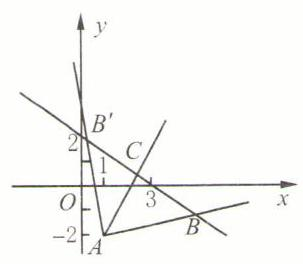
\includegraphics[width=0.2\textwidth]{bodyxb/src/bo_d20aucref24c73anc48g_46_1158_1838_303_264_0.jpg}
\end{center}


(图 7)

例 1 如图 7,等腰直角三角形 ${ABC}$ 的直角顶点 $C$ 和顶点 $B$ 都在直线 ${2x} + {3y} - 6 = 0$ 上,顶点 $A$ 的坐标是(1, - 2),求边 ${AB},{AC}$ 所在的直线方程.

解 $\because {AC} \bot  {BC},\therefore {k}_{AC} = \dfrac{3}{2}$ ,于是可设直线 ${AC}$ 的方程为

${3x} - {2y} + m = 0.$

将点(1, - 2)的坐标代入,得 $m =  - 7$ ,故直线 ${AC}$ 的方程为 ${3x} - {2y} - 7 = 0$ ,

设直线 ${AB}$ 的斜率为 $k$ ,而直线 ${BC}$ 的斜率为 $- \dfrac{2}{3}$ ,故有 $\tan {45}^{ \circ  } = \left| \dfrac{k + \dfrac{2}{3}}{1 - \dfrac{2}{3}k}\right|$ ,即 $\dfrac{{3k} + 2}{3 - {2k}} =  \pm  1$ ,

于是得 $k = \dfrac{1}{5}$ 或 $k =  - 5$ ,故直线 ${AB}$ 的方程为 $y + 2 = \dfrac{1}{5}\left( {x - 1}\right)$ 或 $y + 2 =  - 5\left( {x - 1}\right)$ ,

即 $x - {5y} - {11} = 0$ 或 ${5x} + y - 3 = 0$ .

*2. ${l}_{1}$ 到 ${l}_{2}$ 的角.

已知两直线 ${l}_{1},{l}_{2}$ 交于点 $P$ ,直线 ${l}_{1}$ 绕点 $P$ 依逆时针方向旋转到与 ${l}_{2}$ 重合时所转的角,叫做 ${l}_{1}$ 到 ${l}_{2}$ 的角,我们简称为 “到角”.

假定不垂直的两条直线 ${l}_{1},{l}_{2}$ 的斜率分别为 ${k}_{1},{k}_{2},{l}_{1}$ 到 ${l}_{2}$ 的角为 $\theta$ ,则 $\tan \theta  = \dfrac{{k}_{2} - {k}_{1}}{1 + {k}_{2}{k}_{1}}$ . 显然,“到角” $\theta$ 有可能是钝角.

例 2 如图 8,已知正方形 ${ABCD}$ 的对角线 ${AC}$ 在直线 $x + {2y} -$  $1 = 0$ 上,且顶点 $A\left( {-5,3}\right) ,B\left( {m,0}\right) \left( {m >  - 5}\right)$ ,求顶点 $B,C,D$ 的坐标.

\begin{center}
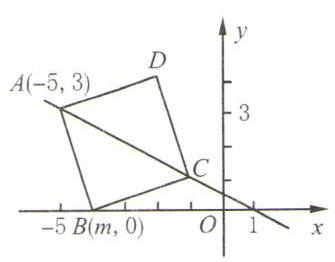
\includegraphics[width=0.2\textwidth]{bodyxb/src/bo_d20aucref24c73anc48g_47_1080_918_335_262_0.jpg}
\end{center}


(图 8)

解 $\because$ 直线 ${AB}$ 到直线 ${AC}$ 的角为 ${45}^{ \circ  }$ ,故由 ${k}_{AB} = \dfrac{-3}{m + 5},{k}_{AC}$  $=  - \dfrac{1}{2}$ ,得 $\tan {45}^{ \circ  } = \dfrac{-\dfrac{1}{2} - \dfrac{-3}{m + 5}}{1 + \left( {-\dfrac{1}{2}}\right) \left( {-\dfrac{3}{m + 5}}\right) }$ ,

化简得 $\dfrac{-m - 5 + 6}{{2m} + {10} + 3} = 1$ ,故 $m =  - 4.\therefore $ 点 $B$ 的坐标为(-4,0).

又 $\because$ 点 $C$ 在直线 $x + {2y} - 1 = 0$ 上,故可设点 $C$ 的坐标为(1 - 2b, b).

由 ${k}_{AB} \cdot  {k}_{BC} =  - 1$ ,得 $\left( {-3}\right)  \cdot  \dfrac{b}{5 - {2b}} =  - 1$ ,故 $b = 1$ ,于是点 $C$ 的坐标为(-1,1).

假设点 $D$ 的坐标为 $\left( {{x}_{0},{y}_{0}}\right) .\because$ 对角线 ${AC}$ 的中点为 $M\left( {-3,2}\right)$ ,故由正方形的对角线互相平分,得 $\left\{  {\begin{array}{l} {x}_{0} + \left( {-4}\right)  =  - 6, \\  {y}_{0} + 0 = 4, \end{array}\therefore \left\{  \begin{array}{l} {x}_{0} =  - 2, \\  {y}_{0} = 4, \end{array}\right. }\right.$ 于是点 $D$ 的坐标为(-2,4).

\section*{【训练题】}

\section*{(A)}

* 55. 若直线 ${l}_{1}$ 的方程为 ${3x} - \sqrt{3}y + 1 = 0$ ,直线 ${l}_{2}$ 的方程为 $\sqrt{3}x - {3y} + 2 = 0$ ,则 ${l}_{1}$ 到 ${l}_{2}$ 的角为(   )

(A) ${150}^{ \circ  }$ . (B) ${120}^{ \circ  }$ . (C) ${60}^{ \circ  }$ . (D) ${30}^{ \circ  }$ .

* 56. 若直线 ${l}_{1} : y = \dfrac{1}{2}x + 2$ ,直线 ${l}_{2}$ 过点 $P\left( {-2,1}\right)$ ,且 ${l}_{1}$ 到 ${l}_{2}$ 的角为 ${45}^{ \circ  }$ ,则 ${l}_{2}$ 的方程为(   )

(A) $y = x - 1$ . (B) $y = \dfrac{1}{3}x + \dfrac{5}{3}$ . (C) $y =  - {3x} + 7$ . (D) $y = {3x} + 7$ .

57. 若直线 $l$ 与直线 ${2x} + y - 1 = 0$ 的夹角为 ${45}^{ \circ  }$ ,则 $l$ 的斜率为 (   )

(A) $- \dfrac{1}{3}$ 或-3. (B) $\dfrac{1}{3}$ 或-3. (C) $- \dfrac{1}{3}$ 或 3. (D) $\dfrac{1}{3}$ 或 3 .

58. 若直线 ${l}_{1}$ 和 ${l}_{2}$ 的斜率是方程 $6{x}^{2} + x - 1 = 0$ 的两根,则 ${l}_{1}$ 与 ${l}_{2}$ 的夹角等于(   )

(A) ${60}^{ \circ  }$ . (B) ${45}^{ \circ  }$ . (C) ${30}^{ \circ  }$ . (D) ${15}^{ \circ  }$ .

59. (1)直线 $x + 1 = 0$ 与 $x + {2y} - 3 = 0$ 的夹角等于\blkda{}；

(2)若直线 ${l}_{1}$ 与 ${l}_{2}$ 的斜率分别是二次方程 ${x}^{2} - \left( {1 - \sqrt{3}}\right) x - \sqrt{3} = 0$ 的两根,则 ${l}_{1}$ 与 ${l}_{2}$ 的夹角等于\blkda{}；

(3)若直线 ${2x} - y = 0$ 与 ${mx} - y = 0$ 的夹角为 ${45}^{ \circ  }$ ,则 $m =$ \blkda{}；

(4)与直线 ${2x} - y + 4 = 0$ 的夹角为 ${45}^{ \circ  }$ ,且与此直线的交点恰好在 $x$ 轴上的直线方程是\blkda{}.

\section*{(B)}

60. 由三条直线 ${3x} - {4y} + {12} = 0,{4x} + {3y} - 9 = 0$ 与 ${14x} - {2y} - {19} = 0$ 所围成的三角形是(   )

(A) 锐角不为 ${45}^{ \circ  }$ 的直角三角形. (B) 顶角不为 ${90}^{ \circ  }$ 的等腰三角形.

(C) 等腰直角三角形. (D) 等边三角形.

61. 已知等腰直角三角形 ${ABC}$ 的斜边所在直线的方程是 ${3x} - y + 2 = 0$ ,直角顶点是 $C(3$ , $- 2)$ ,则两条直角边 ${AC}$ 与 ${BC}$ 的方程分别为(   )

(A) ${2x} + y - 4 = 0,x - {2y} - 7 = 0$ . (B) ${3x} - y + 5 = 0,x + {2y} - 7 = 0$ .

(C) ${2x} - y + 4 = 0,{2x} + y - 7 = 0$ . (D) ${3x} - {2y} - 2 = 0,{2x} - y + 2 = 0$ .

62. (1) 已知直线 ${l}_{1} : {5x} + {2y} + 3 = 0$ ,直线 ${l}_{2}$ 经过点 $P\left( {2,1}\right)$ ,且与 ${l}_{1}$ 的夹角等于 ${45}^{ \circ  }$ ,那么直线 ${l}_{2}$ 的方程为\blkda{}；

$* \left( 2\right)$ 将直线 $x + {2y} + 1 = 0$ 绕着它与 $y$ 轴的交点,按逆时针方向旋转 $\dfrac{\pi }{4}$ ,得到直线 $l$ ,则 $l$ 的方程是\blkda{}.

63. (1) 已知等腰三角形 ${ABC}$ 的底边 ${BC}$ 在直线 $x + y = 0$ 上,顶点为 $A\left( {2,3}\right)$ ,若一腰平行于直线 $x - {4y} + 2 = 0$ ,求另一腰所在直线的方程；

(2)已知等腰三角形的底边过点 $P\left( {2,1}\right)$ ,两腰所在的直线为 $x + y - 2 = 0$ 与 ${7x} - y + 4 =$ 0 ,求其底边所在直线的方程.

\section*{(三) 两条直线的交点}

\section*{【典型题型和解题技巧】}

\section*{1. 两直线交点的逆用.}

求两相交直线 ${l}_{1} : {a}_{1}x + {b}_{1}y + {c}_{1} = 0$ 和 ${l}_{2} : {a}_{2}x + {b}_{2}y + {c}_{2} = 0$ 的交点,只需解方程组 $\left\{  \begin{array}{l} {a}_{1}x + {b}_{1}y + {c}_{1} = 0, \\  {a}_{2}x + {b}_{2}y + {c}_{2} = 0. \end{array}\right.$

从另一个角度来理解,就是 ${l}_{1}$ 和 ${l}_{2}$ 的交点 $\left( {{x}_{0},{y}_{0}}\right)$ 应满足以上方程组. 有一些与两直线交点有关的问题,常常用这种思想方法来求解.

例 1 已知点 $P\left( {-3, - 1}\right) ,Q\left( {4,6}\right)$ ,线段 ${PQ}$ 与直线 ${3x} + {2y} - 5 = 0$ 交于点 $M$ ,求点 $M$ 分 $\vv{PQ}$ 的比.

\begin{center}
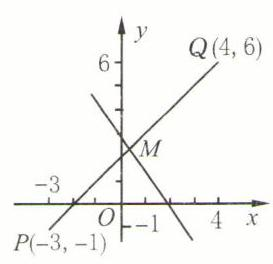
\includegraphics[width=0.2\textwidth]{bodyxb/src/bo_d20aucref24c73anc48g_49_1139_718_273_264_0.jpg}
\end{center}


(图 9)

解 如图 9,设点 $M$ 的坐标为 $\left( {{x}_{0},{y}_{0}}\right) ,\dfrac{\left| PM\right| }{\left| MQ\right| } = \lambda$ ,则 $\left\{  \begin{array}{l} {x}_{0} = \dfrac{-3 + {4\lambda }}{1 + \lambda }, \\  {y}_{0} = \dfrac{-1 + {6\lambda }}{1 + \lambda }. \end{array}\right.$

将 $\left( {{x}_{0},{y}_{0}}\right)$ 的坐标代入 ${3x} + {2y} - 5 = 0$ ,

得 $3 \times  \dfrac{-3 + {4\lambda }}{1 + \lambda } + 2 \times  \dfrac{-1 + {6\lambda }}{1 + \lambda } - 5 = 0$ ,

解得 $\lambda  = \dfrac{16}{19}$ ,即点 $M$ 分 $\vv{PQ}$ 之比为 $\dfrac{16}{19}$ .

例 2 如图 10,已知直线 $l$ 过点 $P\left( {0,1}\right)$ ,并与直线 ${l}_{1} : x - {3y} + {10} = 0$ 和 ${l}_{2} : {2x} + y - 8 = 0$ 分别交于点 $A,B$ . 若线段 ${AB}$ 被点 $P$ 平分,求直线 $l$ 的方程.

分析 ` 直线 $l$ 过点 $P\left( {0,1}\right)$ , $\therefore$ 可设直线 $l$ 的方程为 $y$  $= {kx} + 1$ . 利用解方程组的方法求出点 $A,B$ 的坐标 (含有参数 $k$ ), 再由线段的中点公式求出 $k$ 的值. 这样的解法比较常规,但解的过程显然比较繁冗.

\begin{center}
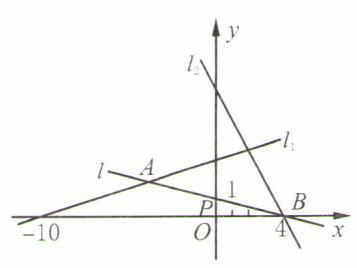
\includegraphics[width=0.3\textwidth]{bodyxb/src/bo_d20aucref24c73anc48g_49_1057_1392_357_268_0.jpg}
\end{center}


(图 10)

我们还可以这样来思考:

$\because$ 点 $B$ 在直线 ${l}_{2} : {2x} + y - 8 = 0$ 上,故我们可以用 “直线标点法”将点 $B$ 表示成为 $B\left( {a,8 - {2a}}\right)$ ,再利用线段的中点公式写出点 $A$ 的坐标 (含有参数 $a$ ),并代入直线 ${l}_{1}$ 的方程.

解 $\because$ 点 $B$ 在直线 ${l}_{2} : {2x} + y - 8 = 0$ 上,故可设 $B$ 的坐标为(a,8 - 2a),

$\because$ 点 $P\left( {0,1}\right)$ 是线段 ${AB}$ 的中点,得点 $A$ 的坐标(-a,2a - 6).

又 $\because$ 点 $A$ 在直线 ${l}_{1} : x - {3y} + {10} = 0$ 上,故将点 $A\left( {-a,{2a} - 6}\right)$ 的坐标代入直线 ${l}_{1}$ 的方程,

得 $- a - 3\left( {{2a} - 6}\right)  + {10} = 0$ ,解得 $a = 4$ .

$\therefore$ 点 $B$ 的坐标是(4,0),因此,过点 $P\left( {0,1}\right) ,B\left( {4,0}\right)$ 的直线 $l$ 的方程为 $\dfrac{x}{4} + \dfrac{y}{1} = 1$ ,

即 $x + {4y} - 4 = 0$ .

2. 两直线位置关系的判断.

假定直线 ${l}_{1}$ 的方程为 $y = {k}_{1}x + {b}_{1}$ (或 ${a}_{1}x + {b}_{1}y + {c}_{1} = 0$ ),直线 ${l}_{2}$ 的方程为 $y = {k}_{2}x + {b}_{2}$ (或 ${a}_{2}x + {b}_{2}y + {c}_{2} = 0$ ), $\left( {{a}_{2},{b}_{2},{c}_{2} \neq  0}\right)$ ,则有:

(1) ${k}_{1} \neq  {k}_{2} \Leftrightarrow  {l}_{1},{l}_{2}$ 相交 $\Leftrightarrow  \dfrac{{a}_{1}}{{a}_{2}} \neq  \dfrac{{b}_{1}}{{b}_{2}}$ ；

(2) ${k}_{1} \cdot  {k}_{2} =  - 1 \Leftrightarrow  {l}_{1} \bot  {l}_{2} \Leftrightarrow  {a}_{1}{a}_{2} + {b}_{1}{b}_{2} = 0$ ；

(3) ${k}_{1} = {k}_{2}$ 且 ${b}_{1} \neq  {b}_{2} \Leftrightarrow  {l}_{1}//{l}_{2} \Leftrightarrow  \dfrac{{a}_{1}}{{a}_{2}} = \dfrac{{b}_{1}}{{b}_{2}} \neq  \dfrac{{c}_{1}}{{c}_{2}}$ ;

(4) ${k}_{1} = {k}_{2}$ 且 ${b}_{1} = {b}_{2} \Leftrightarrow  {l}_{1},{l}_{2}$ 重合 $\Leftrightarrow  \dfrac{{a}_{1}}{{a}_{2}} = \dfrac{{b}_{1}}{{b}_{2}} = \dfrac{{c}_{1}}{{c}_{2}}$ .

例 3 已知直线 ${l}_{1} : x + {my} + 6 = 0$ ,直线 ${l}_{2} : \left( {m - 2}\right) x + {3y} + {2m} = 0$ ,求 $m$ 的值,使得 ${l}_{1}$ 和 ${l}_{2}$ :

(1)相交; (2)垂直； (3) 平行; (4)重合.

解 (1) 当 $m = 0$ 时, ${l}_{1} : x =  - 6,{l}_{2} : {2x} - {3y} = 0$ ,显然 ${l}_{1}$ 和 ${l}_{2}$ 相交.

当 $m \neq  0$ 时,要 ${l}_{1}$ 与 ${l}_{2}$ 相交,只需 $\dfrac{m - 2}{1} \neq  \dfrac{3}{m}$ ,即 ${m}^{2} - {2m} - 3 \neq  0,\therefore m \neq  3$ 且 $m \neq   - 1$ .

(2)要使 ${l}_{1}$ 与 ${l}_{2}$ 垂直,只需 $\left( {m - 2}\right)  \cdot  1 + {3m} = 0,\therefore m = \dfrac{1}{2}$ .

(3) 要使 ${l}_{1}//{l}_{2}$ ,显然 $m \neq  0$ ,故只需 $\dfrac{m - 2}{1} = \dfrac{3}{m} \neq  \dfrac{2m}{6}$ ,即 $\left\{  {\begin{array}{l} {m}^{2} - {2m} - 3 = 0, \\  {m}^{2} - 9 \neq  0, \end{array}\therefore m =  - 1}\right.$ .

(4)要使 ${l}_{1}$ 与 ${l}_{2}$ 重合,由(1)知,显然 $m \neq  0$ ,故只需 $\dfrac{m - 2}{1} = \dfrac{3}{m} = \dfrac{2m}{6}$ ,

即 $\left\{  {\begin{array}{l} {m}^{2} - {2m} - 3 = 0, \\  {m}^{2} - 9 = 0, \end{array}\therefore m = 3}\right.$ .

3. 过两相交直线交点的直线系.

设两相交直线 ${l}_{1},{l}_{2}$ 的方程分别为 ${a}_{1}x + {b}_{1}y + {c}_{1} = 0$ 和 ${a}_{2}x + {b}_{2}y + {c}_{2} = 0$ ,则过 ${l}_{1},{l}_{2}$ 交点的直线系方程为 ${a}_{1}x + {b}_{1}y + {c}_{1} + \lambda \left( {{a}_{2}x + {b}_{2}y + {c}_{2}}\right)  = 0$ . 它包括直线 ${l}_{1}\left( {\lambda  = 0}\right)$ ,但不包括直线 ${l}_{2}$ .

例 4 求过两直线 $x - {2y} + 4 = 0$ 和 $x + y - 2 = 0$ 的交点,且满足下列条件的直线 $l$ 的方程:

(1) 过点(2, - 1);

(2)和直线 ${3x} - {4y} + 5 = 0$ 垂直.

解 可设所求直线 $l$ 的方程为 $x - {2y} + 4 + \lambda \left( {x + y - 2}\right)  = 0$ ,

即 $\left( {\lambda  + 1}\right) x + \left( {\lambda  - 2}\right) y + 4 - {2\lambda } = 0$ .

(1)将点(2, - 1)的坐标代入,得 $2\left( {\lambda  + 1}\right)  - \left( {\lambda  - 2}\right)  + 4 - {2\lambda } = 0$ ,故 $\lambda  = 8$ .

$\therefore$ 直线 $l$ 的方程为 ${3x} + {2y} - 4 = 0$ .

(2)由直线互相垂直的条件,得 $3\left( {\lambda  + 1}\right)  - 4\left( {\lambda  - 2}\right)  = 0$ ,故 $\lambda  = {11}$ .

$\therefore$ 直线 $l$ 的方程为 ${4x} + {3y} - 6 = 0$ .

例 5 求证: 不论 $m$ 取何实数,直线 $\left( {{2m} - 1}\right) x - \left( {m + 3}\right) y - \left( {m - {11}}\right)  = 0$ 恒过一个定点, 并求此定点的坐标.

证法一 将直线方程变形为 $\left( {x + {3y} - {11}}\right)  - m\left( {{2x} - y - 1}\right)  = 0$ ,

它表示过两直线 $x + {3y} - {11} = 0$ 和 ${2x} - y - 1 = 0$ 交点的直线系,解方程组 $\left\{  {\begin{array}{l} x + {3y} - {11} = 0, \\  {2x} - y - 1 = 0, \end{array}\text{ 得 }\left\{  \begin{array}{l} x = 2, \\  y = 3. \end{array}\right. }\right.$

$\therefore$ 上述直线恒过定点(2,3).

证法二 在直线方程中,令 $m = \dfrac{1}{2}$ ,得 $y = 3$ ; 再令 $m =  - 3$ ,得 $x = 2$ .

两直线 $x = 2$ 和 $y = 3$ 的交点为(2,3),将点(2,3)的坐标代入直线方程左边:

$2\left( {{2m} - 1}\right)  - 3\left( {m + 3}\right)  - \left( {m - {11}}\right)  = \left( {{4m} - {3m} - m}\right)  - \left( {2 + 9 - {11}}\right)  = 0,$

因此,已知直线恒过定点(2,3).

\section*{【训练题】}

\section*{(A)}

64. 若三条直线 ${2x} + {3y} + 8 = 0,x - y - 1 = 0$ 和 $x + {ky} = 0$ 相交于一点,则 $k$ 的值等于(   )

(A) -2 . (B) $- \dfrac{1}{2}$ . (C) 2 . (D) $\dfrac{1}{2}$ .

65. 若直线 ${5x} + {4y} = {2m} + 1$ 与直线 ${2x} + {3y} = m$ 的交点在第四象限,则 $m$ 的取值范围是(   )

(A) $m < 2$ . (B) $m > \dfrac{3}{2}$ . (C) $m <  - \dfrac{3}{2}$ . (D) $- \dfrac{3}{2} < m < 2$ .

66. 下列说法中,正确的是(   )

(A) 若直线 ${l}_{1}$ 与 ${l}_{2}$ 的斜率相等,则 ${l}_{1}//{l}_{2}$ .

(B) 若直线 ${l}_{1}$ 与 ${l}_{2}$ 互相平行,则它们的斜率相等.

(C) 直线 ${l}_{1}$ 与 ${l}_{2}$ 中,若一条直线的斜率存在,另一条直线的斜率不存在,则 ${l}_{1}$ 与 ${l}_{2}$ 一定相交.

(D) 若直线 ${l}_{1}$ 与 ${l}_{2}$ 的斜率都不存在,则 ${l}_{1}//{l}_{2}$ .

67. 若直线 $\left( {2{m}^{2} + m - 3}\right) x + \left( {{m}^{2} - m}\right) y = {4m} - 1$ 与直线 ${2x} - {3y} = 5$ 互相平行,则 $m$ 的值等于(   )

(A) $- \dfrac{3}{2}$ 或 1 . (B) $- \dfrac{9}{8}$ 或 1. (C) $- \dfrac{9}{8}$ . (D) 1 .

68. 直线 ${3x} - {2y} + m = 0$ 和 $\left( {{m}^{2} + 1}\right) x + {3y} - {3m} = 0$ 的位置关系是(   )

(A) 平行. (B) 重合. (C) 相交. (D) 不确定.

69. 已知直线 ${l}_{1} : \left( {a + 2}\right) x + \left( {a + 3}\right) y = 5$ 与 ${l}_{2} : {6x} + \left( {{2a} - 1}\right) y = 5$ .

(1)若 ${l}_{1}$ 与 ${l}_{2}$ 重合,则 $a =$ \blkda{}；

(2)若 ${l}_{1}$ 与 ${l}_{2}$ 互相平行,则 $a =$ \blkda{}；

(3)若 ${l}_{1}$ 与 ${l}_{2}$ 互相垂直,则 $a =$ \blkda{}.

70. (1) 若直线 ${mx} + {2y} - 1 = 0$ 与直线 ${2x} - {5y} + n = 0$ 垂直且相交于点(1, a),则 $m =$ \blkda{}, $n =$ \blkda{}, $a =$ \blkda{};

$* \left( 2\right)$ 若直线 ${l}_{1} : {ax} + {2y} + 2 = 0$ 与 ${l}_{2} : {2x} + {6y} + c = 0$ 相交于点(1, m),且 ${l}_{2}$ 到 ${l}_{1}$ 的角为 ${45}^{ \circ  }$ ,则 $a =$ \blkda{}, $c =$ \blkda{}, $m =$ \blkda{}.

\section*{(B)}

71. 两直线 $x - \sqrt{3}y = 0$ 与 $x - 1 = 0$ 夹角的平分线方程是 (   )

(A) ${3x} - \sqrt{3}y - 2 = 0$ . (B) ${3x} - \sqrt{3}y + 2 = 0$ .

(C) ${3x} - \sqrt{3}y + 2 = 0$ 或 $x + \sqrt{3}y - 2 = 0$ . (D) $x + \sqrt{3}y - 2 = 0$ .

72. 若方程 $y = a\left| x\right|$ 和 $y = x + a\left( {a > 0}\right)$ 所确定的曲线有两个交点,则 $a$ 的取值范围是(   )

(A) $a > 1$ . (B) $0 < a < 1$ 或 $a > 1$ .

(C) $0 < a < 1$ . (D) $a > 0$ .

73. 若直线 ${a}_{1}x + {b}_{1}y + 1 = 0$ 与 ${a}_{2}x + {b}_{2}y + 1 = 0$ 的交点是 $P\left( {2,3}\right)$ ,则过两点 ${Q}_{1}\left( {{a}_{1},{b}_{1}}\right)$ , ${Q}_{2}\left( {{a}_{2},{b}_{2}}\right)$ 的直线方程是 (   )

(A) ${3x} + {2y} = 0$ . (B) ${2x} - {3y} + 5 = 0$ .

(C) ${2x} + {3y} + 1 = 0$ . (D) ${3x} + {2y} + 1 = 0$ .

74. 已知三条直线 ${4x} + y - 4 = 0,{mx} + y = 0$ 和 ${2x} - {3my} - 4 = 0$ ,求符合下列条件时 $m$ 的值.

(1)使这三条直线相交于同一点；

(2)使这三条直线不能构成三角形.

75. 已知菱形 ${ABCD}$ 的一边 ${AB}$ 所在直线的方程为 $x - y + 4 = 0$ ,一对角线端点为 $A\left( {-2,2}\right)$ , $C\left( {4,4}\right)$ ,求菱形另三边所在直线的方程.

76. (1) 过点 $P\left( {2,2}\right)$ 作直线 $l$ ,使 $l$ 夹在两直线 ${2x} - y + 1 = 0$ 与 $x - {3y} - 2 = 0$ 之间的线段被点 $P$ 平分,求直线 $l$ 的方程;

(2)已知点 $A\left( {3, - 5}\right) ,B\left( {5,2}\right)$ ,直线 $x - y - 2 = 0$ 交直线 ${AB}$ 于点 $P$ ,求点 $P$ 分 $\vv{AB}$ 的比 $\lambda$ ；

(3)已知 $M\left( {{x}_{1},{y}_{1}}\right) ,N\left( {{x}_{2},{y}_{2}}\right)$ 是直线 $l : {ax} + {by} + c = 0$ 外的两点,且直线 ${MN}$ 交 $l$ 于点 $P$ ,求点 $P$ 分 $\vv{MN}$ 的比 $\lambda$ .

77. (1) 已知入射光线沿 ${2x} - y + 1 = 0$ 射向直线 $x - y = 0$ 后反射,求反射光线所在的直线方程；

(2)求直线 ${l}_{1} : x - y - 2 = 0$ 关于直线 ${l}_{2} : {3x} - y + 3 = 0$ 对称的直线方程；

(3)已知 $\bigtriangleup  {ABC}$ 的三条边所在直线方程分别是 ${AB} : {4x} - {3y} + {10} = 0,{BC} : y - 2 = 0,{CA}$ : ${3x} - {4y} - 5 = 0$ ,试求 $\angle {BAC}$ 的平分线所在的直线方程.

78. (1) 求过两直线 ${3x} - {2y} + 5 = 0$ 和 ${5x} + {4y} - 3 = 0$ 的交点,且过定点 $P\left( {1,3}\right)$ 的直线 $l$ 的方程;

(2)求过两直线 ${3x} + y - 5 = 0$ 和 ${2x} - {3y} + 4 = 0$ 的交点,且在两坐标轴上截距相等的直线方程.

\section*{(四) 点到直线的距离}

\section*{【典型题型和解题技巧】}

例 如图 11,已知直线 $l$ 过点 $P\left( {1,2}\right)$ ,且被两平行直线 ${l}_{1} : {4x} + {3y} + 1 = 0$ 与 ${l}_{2} : {4x} + {3y} +$  $6 = 0$ 截得的线段长为 $\sqrt{2}$ ,求直线 $l$ 的方程.

解 平行直线 ${l}_{1} : {4x} + {3y} + 1 = 0$ 与 ${l}_{2} : {4x} + {3y} + 6 = 0$ 间的距离为 $\left| {AC}\right|  = \dfrac{\left| 6 - 1\right| }{\sqrt{{4}^{2} + {3}^{2}}} = 1$ ,而 $\left| {AB}\right|  = \sqrt{2}$ ,故直线 $l$ 与 ${l}_{1},{l}_{2}$ 的夹角都为 ${45}^{ \circ  }$ . 设 $l$ 的斜率为 $k$ ,则 $\tan {45}^{ \circ  } = \left| \dfrac{k + \dfrac{4}{3}}{1 - \dfrac{4}{3}k}\right|$ ,即 $\left| {{3k} + 4}\right|  = \left| {{4k} - 3}\right|$ ,解得 ${k}_{1} =  - \dfrac{1}{7}$ , ${k}_{2} = 7$ . 故直线 $l$ 的方程为 $x + {7y} - {15} = 0$ 和 ${7x} - y - 5 = 0$ .

\begin{center}
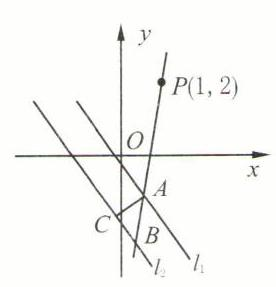
\includegraphics[width=0.2\textwidth]{bodyxb/src/bo_d20aucref24c73anc48g_53_1132_715_276_287_0.jpg}
\end{center}


(图 11)

\section*{【训练题】}

\section*{(A)}

79. 若 $p <  - 1$ ,则点 $\left( {\cos \theta ,\sin \theta }\right)$ 到直线 $x\cos \theta  + y\sin \theta  + p = 0$ 的距离等于(   )

(A) $1 + p$ . (B) $1 - p$ .

(C) $- 1 + p$ . (D) $- 1 - p$ .

80. 已知直线 ${3x} + {2y} - 3 = 0$ 与 ${6x} + {my} + 1 = 0$ 互相平行,则它们之间的距离等于 (   )

(A) 4. (B) $\dfrac{2}{13}\sqrt{13}$ . (C) $\dfrac{5}{26}\sqrt{13}$ . (D) $\dfrac{7}{26}\sqrt{13}$ .

81. 已知点 $A\left( {-6,0}\right) ,B\left( {0,8}\right)$ ,点 $P$ 在线段 ${AB}$ 上,且 $\left| {AP}\right|  : \left| {AB}\right|  = 3 : 5$ ,则点 $P$ 到直线 ${15x} + {20y} - {16} = 0$ 的距离为(   )

(A) $\dfrac{44}{25}$ . (B) $\dfrac{49}{100}$ . (C) $\dfrac{6}{25}$ . (D) $\dfrac{12}{25}$ .

82. ( 1 )已知 $A,B,C$ 三点的坐标分别是 $A\left( {5,7}\right) ,B\left( {-4,6}\right) ,C\left( {8, - 3}\right)$ ,则点 $A$ 到直线 ${BC}$ 的距离 $d =$ \blkda{}；

(2)若点 $P\left( {2,3}\right)$ 到直线 ${ax} + \left( {a - 1}\right) y + 3 = 0$ 的距离等于 3,则 $a$ 的值等于\blkda{}；

(3)已知直线 $l$ 平行于直线 $x + y + 2 = 0$ ,且这两条直线之间的距离为 $3\sqrt{2}$ ,则直线 $l$ 的方程为\blkda{}；

(4)已知 $0 \leq  \theta  \leq  \dfrac{\pi }{2}$ ,且点 $\left( {1,\cos \theta }\right)$ 到直线 $x\sin \theta  + y\cos \theta  = 1$ 的距离为 $\dfrac{1}{4}$ ,则 $\theta$ 的值等于\blkda{}；

(5)点 $P\left( {1,1}\right)$ 到直线 $x\cos \theta  + y\sin \theta  - 2 = 0$ 的最小距离是\blkda{},最大距离是\blkda{}；

(6)到原点和直线 $x + {3y} - 2 = 0$ 的距离相等且又在直线 $x + {3y} = 0$ 上的点 $P$ 的坐标是\blkda{}.

\section*{(B)}

83. 过点(1,3)且与原点相距为 1 的直线共有(   )

(A) 3 条. (B) 2 条. (C) 1 条. (D) 0 条.

84. 已知两点 $O\left( {0,0}\right) ,A\left( {4, - 1}\right)$ 到直线 ${mx} + {m}^{2}y + 6 = 0$ 的距离相等,则实数 $m$ 可取的不同值共有(   )

(A) 1 个. (B) 2 个. (C) 3 个. (D) 4 个.

85. 过点(3,4)且与两点 $\left( {4, - 2}\right) ,\left( {-2,2}\right)$ 等距离的直线方程是 (   )

(A) ${2x} + {3y} - {18} = 0$ 和 ${2x} + y - 2 = 0$ . (B) ${3x} - {2y} + {18} = 0$ 和 $x + {2y} + 2 = 0$ .

(C) ${2x} + {3y} - {18} = 0$ 和 ${2x} - y - 2 = 0$ . (D) ${3x} - {2y} + {18} = 0$ 和 ${2x} - y - 2 = 0$ .

86. 已知两平行直线 ${l}_{1} : {3x} + {4y} - {10} = 0$ 和 ${l}_{2} : {3x} + {4y} - {25} = 0$ ,又直线 $l$ 和 ${l}_{1}$ 之间的距离与 $l$ 和 ${l}_{2}$ 之间的距离之比为 $2 : 3$ ,求直线 $l$ 的方程.

87. (1) 已知直线 ${l}_{1} : {5x} - {2y} + {3m}\left( {{3m} + 1}\right)  = 0$ 与 ${l}_{2} : {2x} + {6y} - {3m}\left( {{9m} + {20}}\right)  = 0$ ,当 $m$ 为何值时,两直线 ${l}_{1},{l}_{2}$ 的交点到直线 ${4x} - {3y} - {12} = 0$ 的距离最小? 这个最小值是多少?

(2)要使三点 $A\left( {1,2}\right)$ , $B\left( {3,1}\right)$ , $C\left( {2,3}\right)$ 到直线 $x - {my} = 0$ 的距离平方和取最大值,实数 $m$ 的值应是多少?

(3)若点 $P\left( {a,b}\right)$ 在直线 $x + y + 1 = 0$ 上,求 $\sqrt{{a}^{2} + {b}^{2} - {2a} - {2b} + 2}$ 的最小值；

(4)在直线 $y =  - {2x} + 4$ 上选一点 $P$ ,在抛物线 $y = 1 - {x}^{2}$ 上选一点 $Q$ ,要使 $\left| {PQ}\right|$ 最小,求点 $P,Q$ 的坐标.

88. (1) 已知两平行直线 ${l}_{1},{l}_{2}$ 分别过点 ${P}_{1}\left( {1,0}\right)$ 与 ${P}_{2}\left( {0,5}\right)$ ,

①若 ${l}_{1}$ 与 ${l}_{2}$ 的距离为 5,求 ${l}_{1},{l}_{2}$ 的方程,

② 设 ${l}_{1}$ 与 ${l}_{2}$ 之间的距离为 $d$ ,求 $d$ 的取值范围；

(2)已知直线 ${l}_{1}$ 和 ${l}_{2}$ 在 $x$ 轴上的截距相等,且它们的倾斜角互补,又直线 ${l}_{1}$ 过点 $P\left( {-3,3}\right)$ . 如果点 $Q\left( {2,2}\right)$ 到 ${l}_{2}$ 的距离为 1,求 ${l}_{2}$ 的方程.

89. 直线 $l$ 过点 $M\left( {2,3}\right)$ ,且被 ${3x} + {4y} - 7 = 0$ 与 ${3x} + {4y} + 8 = 0$ 截得的线段长为 $3\sqrt{2}$ ,求直线 $l$ 的方程.

90. 已知 ${a}^{2}\sin \theta  + a\cos \theta  - 1 = 0,{b}^{2}\sin \theta  + b\cos \theta  - 1 = 0\left( {a \neq  b}\right)$ . 求证: 无论 $a,b$ 取何实数,坐标原点到经过两点 $\left( {a,{a}^{2}}\right) ,\left( {b,{b}^{2}}\right)$ 的直线的距离为定值.

\section*{(C)}

91. 已知点 $M\left( {2,3}\right) ,N\left( {8,4}\right)$ ,点 $P$ 在线段 ${MN}$ 上,且 $\dfrac{\left| MP\right| }{\left| PN\right| } = \dfrac{\left| PN\right| }{\left| MN\right| }$ . 求点 $P$ 的坐标.

92. 已知 $a\cos \alpha  + b\sin \alpha  = c,a\cos \beta  + b\sin \beta  = c\left( {\alpha  \pm  \beta  \neq  {k\pi },k \in  \mathbf{Z}}\right)$ ,试利用两直线位置关系的知识证明: $\dfrac{a}{\cos \dfrac{\alpha  + \beta }{2}} = \dfrac{b}{\sin \dfrac{\alpha  + \beta }{2}} = \dfrac{c}{\cos \dfrac{\alpha  - \beta }{2}}$ .

93. $A\left( {-1,1}\right)$ 和 $B\left( {1,1}\right)$ 是直线 $x - y - 2 = 0$ 外的两个定点,试在已知直线上找一点 $P$ ,使 $\angle {APB}$ 最大.

94. 已知集合 $A = \left\{  {\left( {x,y}\right) \left| {\dfrac{y - 3}{x - 2} = a + 1}\right. }\right\}$ 与 $B = \left\{  {\left( {x,y}\right) \left| {\left( {{a}^{2} - 1}\right) x + \left( {a - 1}\right) y = {15}}\right. }\right\}$ 满足 $A \cap  B = \varnothing$ ,求实数 $a$ 的值.

95. 在 $\bigtriangleup {ABC}$ 中,已知顶点 $A$ 的坐标是 $A\left( {1,4}\right) ,\angle {ABC}$ 与 $\angle {ACB}$ 的平分线所在的直线方程分别为 $x - {2y} = 0$ 与 $x + y - 1 = 0$ ,求直线 ${BC}$ 的方程.

96. 已知两定点 $A\left( {-3, - 8}\right) ,B\left( {{10},4}\right)$ 及两平行直线 ${l}_{1} : {3x} + {4y} + {10} = 0,{l}_{2} : {3x} + {4y} - {15} = 0$ , 试在 ${l}_{1},{l}_{2}$ 上分别求点 $P,Q$ ,使得 ${PQ} \bot  {l}_{1}$ ,且折线段 ${APQB}$ 的长度最短,并写出此时三条折线所在直线的方程.

97. 直线 ${l}_{1} : y = {mx} + 1$ 和 ${l}_{2} : x =  - {my} + 1$ 相交于点 $P$ ,其中常数 $m$ 满足 $\left| m\right|  < 1$ ,

(1)求证: ${l}_{1},{l}_{2}$ 分别过定点 $A,B$ ；

(2)用 $m$ 表示点 $P$ 的坐标；

(3)用 $m$ 表示 $\bigtriangleup  {ABP}$ 的面积 $S$ ；

(4)当 $m$ 为何值时,面积 $S$ 最大? 并求出这个最大值.

98. 若方程 $a{x}^{2} - {4xy} + \sqrt{3}{y}^{2} + 3\sqrt{3}x - {3y} = 0$ 表示两条直线,求实数 $a$ 的值.

99. 若直线 $y = {mx}$ 与函数 $y = \dfrac{\left| x\right|  - 1}{\left| x - 1\right| }$ 的图像没有公共点,求实数 $m$ 的取值范围.

100. 已知函数 $y = \left( {x - 1}\right) {\log }_{3}^{2}a - 6{\log }_{3}a \cdot  x + x + 1$ 在 $x \in  \left\lbrack  {0,1}\right\rbrack$ 内恒正,求 $a$ 的取值范围.

101. 用解析法证明:

\begin{center}
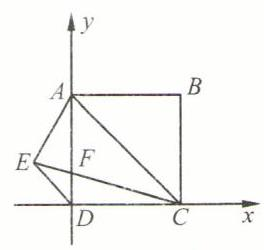
\includegraphics[width=0.2\textwidth]{bodyxb/src/bo_d20aucref24c73anc48g_55_1147_1401_264_250_0.jpg}
\end{center}


[第 101(2)题]

(1)两条中线相等的三角形是等腰三角形；

(2)过正方形 ${ABCD}$ 的顶点 $D$ 作对角线 ${AC}$ 的平行线 ${DE}$ ,使 $\left| {CE}\right|$  $= \left| {AC}\right| ,{CE}$ 与 ${AD}$ 交于点 $F$ (如图),求证: $\left| {AF}\right|  = \left| {AE}\right|$ .

102. (1) 已知直线方程 ${2x} - y - 6 + \lambda \left( {x - y - 4}\right)  = 0$ ,求证: 无论 $\lambda$ 取何实数,此直线与点 $P\left( {3, - 1}\right)$ 的距离恒不等于 3 ;

(2)求证:无论 $k$ 取何值,直线 $\left( {2 + k}\right) x - \left( {1 + k}\right) y - 2\left( {3 + {2k}}\right)  = 0$ 与点 $P\left( {-2,2}\right)$ 的距离 $d$ 都不能大于或等于 $4\sqrt{2}$ .

103. 求证下列直线恒过定点, 并求此定点:

(1)直线 $\left( {m - 1}\right) x + \left( {{2m} - 1}\right) y = m - 5\left( {m \in  \mathbf{R}}\right)$ ；

(2)直线 ${px} + {3y} + q = 0$ ,其中 $p$ , $q$ 满足 $p + {2q} - 1 = 0$ ；

(3)已知直线 $\left( {{2m} + n}\right) x + \left( {{3m} - {2n}}\right) y - {18m} + {5n} = 0$ ,其中 $m,n$ 是不同时为零的实数.

